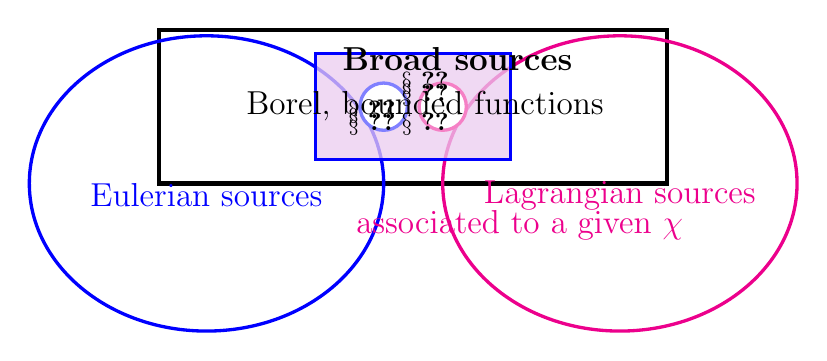
\begin{tikzpicture}[scale=0.75]
% Set up the bounding box
\draw[black, ultra thick] (-4.3,-1.3) rectangle (4.3, 1.3);
% Set up the ellipses
\draw[blue, very thick] (-3.5,-1.3) ellipse (3cm and 2.5cm);
\draw[magenta, very thick] (3.5,-1.3) ellipse (3cm and 2.5cm);
% Set up the intersection area
\filldraw[blue!20, fill opacity=0.5, draw=magenta, very thick] (-1.65,-0.9)--(-1.65,0.9)--(1.65,0.9)--(1.65,-0.9)--cycle;
\filldraw[magenta!20, fill opacity=0.5, draw=blue, very thick] (1.65,-0.9)--(1.65,0.9)--(-1.65,0.9)--(-1.65,-0.9)--cycle;

% Set up the circles
\filldraw[fill=white, draw=blue!50, very thick] (-0.5,0) circle (0.4cm);
\filldraw[fill=white, draw=magenta!50, very thick] (0.5,0) circle (0.4cm);

% Set up the labels
\node at (0.75,0.8) {\large \bfseries Broad sources};
\node at (-3.5,-1.5) {\large \textcolor{blue}{Eulerian sources}};
\node at (3.5,-1.5) {\large \textcolor{magenta}{Lagrangian sources}};
\node at (1.8,-2) {\large \textcolor{magenta}{associated to a given $\chi$}};
\node at (0.2,0.4) {\small $\S$ \ref{sec:Borel}};
\node at (-0.7,-0.1) {\small $\S$ \ref{sec:Borel}};
\node at (0.2,0.2) {\small $\S$ \ref{sec:Borel}};
\node at (-0.7,-0.3) {\small $\S$ \ref{sec:Borel}};
\node at (0.2,-0.3) {\small $\S$ \ref{sec:Borel}};
\node at (0.2,0.0) {\large Borel, bounded functions};
\end{tikzpicture}